\chapter{Aufgabenstellung}\label{ch:aufgabenstellung}
In diesem Kapitel ist die Aufgabenstellung der Probe-IPA aufgeführt. Die Inhalte wurden zu einem grossen Teil von der originalen Aufgabenstellung übernommen und Angepasst.

\section{Ausgangslage}\label{sec:ausgangslage}
Die Firma \gls{Ergon Informatik AG} entwickelt sein einigen Jahren eine Transaktions-Authorisierungs-Lösung für einige Banken in der Schweiz. Dieses Projekt heisst \gls{CardX} und wird durch ein 12 zwölfköpfiges Team umgesetzt. In diesem Projekt ist der Lernende seit Januar 2024 tätig und kennt sich deshalb schon ein bisschen aus.

Das Projekt kommuniziert mit verschiedenen bankspeziefischen IT-Systemen wie zum Beispiel dem Kernbankensystem oder Service-Büros über Message-Queues. Diese Message-Queues werden in der Datenbank-Tabelle MQ\_TABLE (eingehende Nachrichten) und MQ\_OUT (ausgehende Nachrichten) zwischengespeichert. Falls man diese Message-Queues anschauen oder bearbeiten möchte, muss man dies in der Datenbank machen. Weil das ziemlich umständlich ist, besteht die Aufgabe des Lernenden jetzt daraus diese Message-Queues in einem \gls{Web-GUI} darzustellen und sinnvolle Interaktionen mit diesen Daten anzubieten.

\section{Detaillierte Aufgabenstellung}\label{sec:detaillierte-aufgabenstellung}

\paragraph{Minimalanforderungen}
Das Ziel dieser Aufgabe ist es, den Inhalt der Tabelle MQ\_TABLE in diesem Web-GUI sichtbar zu machen und dem Nutzer sinnvolle Interaktionen mit diesen Daten anzubieten.

Es soll im Weg-GUI eine neue Seite erstellt werden mit dem Inhalt einer Tabelle, welche die Message-Queues abbilden soll. Die Tabelle soll eine Hand voll Spalten besitzen, sodass sie übersichtlicher ist. Die Seite soll stimmig in das \gls{UI} eingebaut werden. Im \gls{Backend} sollen die neuen Methoden mithilfe von Unit-Tests abgedeckt werden.

Zusätzlich kann der Lernende noch zwischen zwei Erweiterungen entscheiden, welche er implementieren möchte.

\paragraph{Erweiterung: Pagination}
Bei der ersten Erweiterungen ist das Ziel ein Paginator zur Tabelle hinzuzufügen. Eine Pagination ist wenn man eine Liste oder Tabelle auf ein paar Einträge limitiert und anschliessend weitere Einträge anzeigen kann mit einer Pfeiltaste. Dies hilft, das Laden der Seite zu verkürzen, da die Einträge, die nicht angezeigt werden, erst geladen werden, wenn sie auch wirklich gebraucht werden.

\paragraph{Erweiterung: Filter}
Die zweite Erweiterung ist ein Filtersystem. Die Seite soll nach dem Status, Inhalt der Nachricht und dem Datum gefiltert werden können. Die Filter-Werte sollen ausserdem in der URL Abgebildet werden, um das Teilen von gefilterten Ergebnissen zu vereinfachen oder den Filter als Lesezeichen abgelegen zu können.

\section{Mittel und Methoden}\label{sec:mittel-und-methoden}

\paragraph{Technologien}
\begin{itemize}
	\item SQL
    \item Java
    \item TypeScript
    \item HTML
    \item Angular
\end{itemize}

\paragraph{Tools}
\begin{itemize}
	\item IntelliJ (IDE)
    \item Docker
	\item Bitbucket
	\item Confluence
	\item Jira
	\item Postman
\end{itemize}

\section{Vorkenntnisse}\label{sec:vorkenntnisse}
Der Lernende hat bereits viele Arbeiten im Projekt CardX gemacht. Unter anderem im Backend und an CardX-spezifischen Tools. Die Codebasis hat der Lernende in den letzten 9 Monaten gut kennengelernt und findet sich gut zurecht. Der Lernende hat auch bereits die Tabelle TASK von der Datenbank in das Web-GUI gebracht, was eine ähnliche Aufgabe war wie die jetzige Aufgabenstellung.

Durch die früheren Projekte, wie ein Fussballtippspiel und eine Anmelde-Plattform für Bewerbende, konnte er bereits viel Erfahrung mit Java und Angular sammeln.

\section{Vorarbeiten}\label{sec:vorarbeiten}
Durch das bereits existierende Projekt und die vielen Arbeiten, die der Lernende bereits gemacht hat, musste er keine Vorarbeiten leisten.

\section{Neue Lerninhalte}\label{sec:neue-lerninhalte}
\begin{itemize}
    \item Pagination: 
    
    Mit Pagination hat der Lernende sich noch nie auseinandergesetzt. Er hat es schon oft auf anderen Seiten gesehen aber noch nie selbst implementiert.
    \item Filtersystem:
    
    Im Projekt WM-Tippspiel gab es ein Filtersystem, aber dieses hat der Lernende nicht selbst implementiert und ist so ein neuer Lerninhalt.
\end{itemize}

\section{Arbeiten in den letzten 6 Monaten}\label{sec:arbeiten-in-den-letzten-6-monaten}
In den letzten 6 Monaten hat der Lernende sich, wie oben schon genannt, mit dem Projekt CardX auseinandergesetzt und ist ein aktives Team Mitglied. Er hat viele verschiedene Arbeiten umgesetzt. Einige davon hier:
\begin{itemize}
    \item CheckDB Task:
    
    In dieser Aufgabe geht es darum, eine Aufgabe zu erstellen, welche periodisch oder manuell ausgeführt werden kann. Diese Aufgabe überprüft die Datenbankdefinition, ob immer noch alles fehlerfrei ist. Es werden Sequenzen, Indexe, Felder und mehr in eine Datei geschrieben, gespeichert und anschliessend mit der vorherigen Datei auf Veränderungen verglichen. Bei einer Veränderung schlägt die Aufgabe fehl und die Differenz wird in der Fehlermeldung angezeigt.
    \item ServiceLogMove und Zip:
    
    Mit der Aufgabe ServiceLogMerge werden Protokolle des Systems in Dateien geschrieben und gespeichert. Ein Teil dieser Dateien wird jetzt mithilfe der Aufgabe in bestimmte Verzeichnisse verschoben und komprimiert. Die Dateien werden nach Bank sortiert und anschliessend in ihn vorgesehenes Verzeichnis verschoben. Auch diese Aufgabe wird periodisch jeden Tag ausgeführt, um die Dateiablage übersichtlich zu halten.
    \item Tasks im Frontend anzeigen und bearbeiten:
    
    Diese Aufgabe zeigt alle Tasks im Frontend an und man kann sie dort auch bearbeiten. Das Ziel von dieser Aufgabe war gleich wie die Mindestanforderungen von der Aufgabenstellung.
    \begin{figure}[H]
    	\begin{center}
    		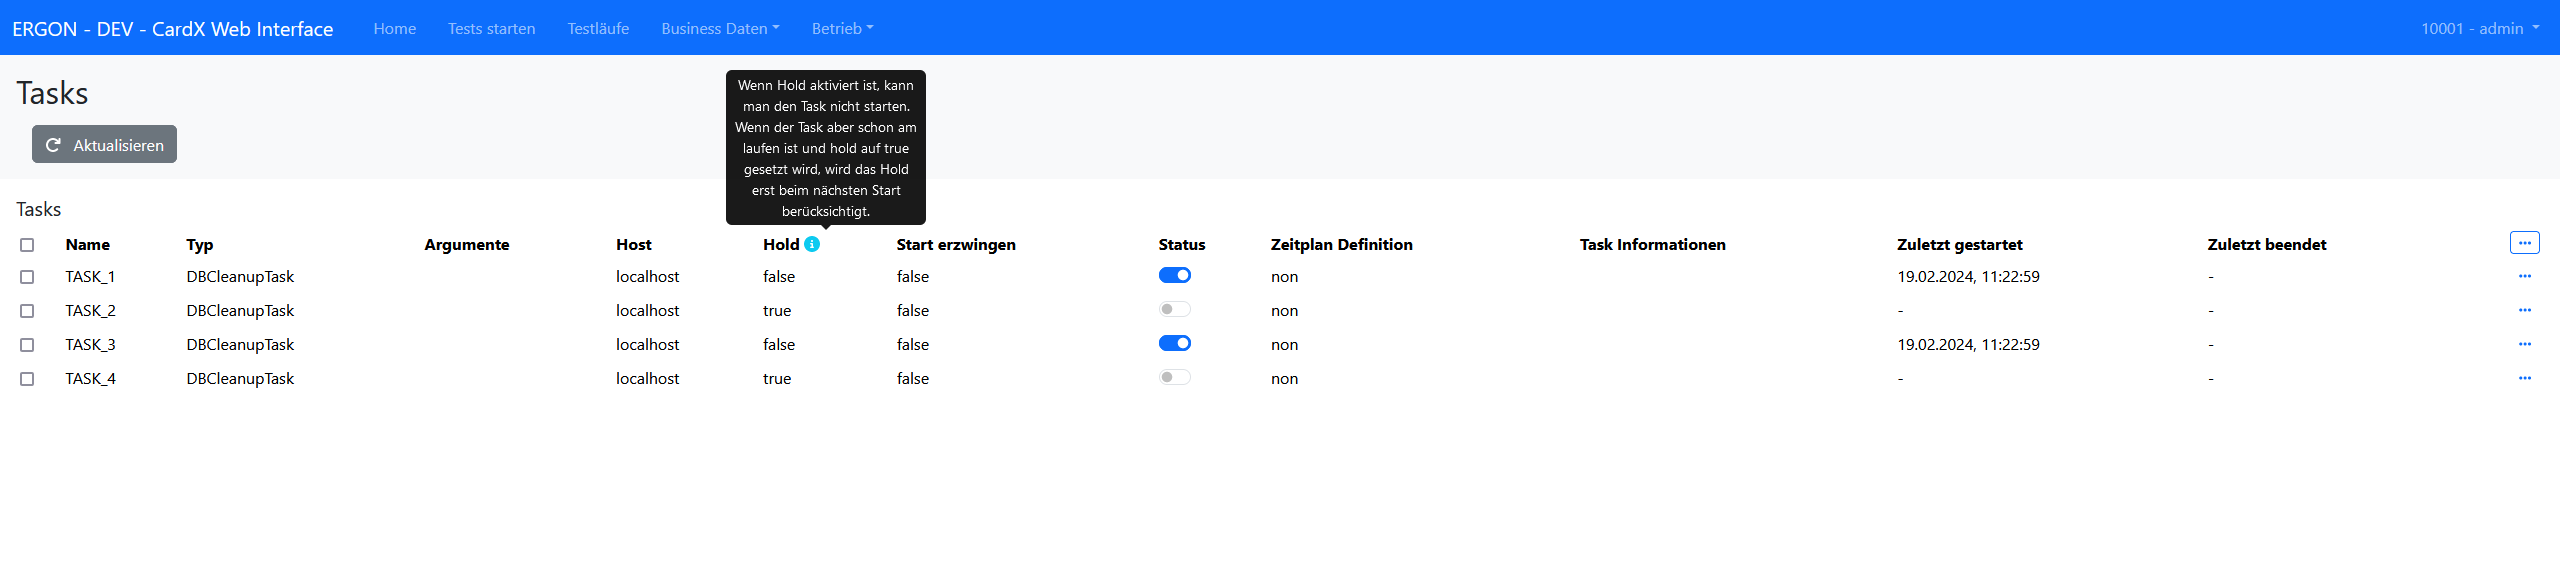
\includegraphics[width=1\textwidth]{ressourcen/show-and-edit-tasks}
    		\caption[Anzeigen und bearbeiten der Tasks]{Anzeigen und bearbeiten der Tasks}\label{fig:show-and-edit-tasks}
    	\end{center}
    \end{figure}
\end{itemize}
